\documentclass[tikz,border=5pt]{standalone}
\usepackage[dvipsnames]{xcolor}
\usepackage{tikz}
\usetikzlibrary{arrows.meta,calc,positioning,bending,quotes,fit}

\tikzset{
  filtered/.style={
    thick,
    ->,
    >=Latex,
    draw=black!30,
    fill=black!30,
    dashed
  },
  sccbox/.style={
    draw=red!70!black,
    fill=red!10,
    dashed,
    rounded corners=4pt,
    inner sep=6pt
  },
  gnode/.style={
    circle,
    draw=blue!50!black,
    fill=blue!12,
    minimum size=12mm,
    inner sep=0pt,
    font=\Large\bfseries
  },
  gnode ghost/.style={
    circle,
    draw=black!35,
    dashed,
    fill=gray!10,
    text=black!45,
    minimum size=12mm,
    inner sep=0pt,
    font=\Large\bfseries
  },
  connection/.style={
    thick,
    ->,
    >=Latex
  },
  glabel/.style={
    draw=black!55,
    line width=0.3pt,
    fill=white,
    rounded corners=1.5pt,
    font=\small,
    inner sep=3pt,
    outer sep=3pt
  },
  every edge quotes/.append style=glabel
}

\begin{document}
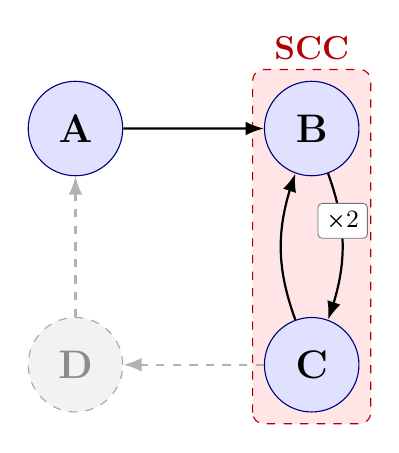
\begin{tikzpicture}
  %\draw[help lines, step=0.5] (-1,-1) grid (6,4);

  % SCC highlight (merge of panel c)
  \draw[sccbox] (2.25,-0.75) rectangle (3.75, 3.75);
  \node[text=red!70!black] at (3,3.75) [anchor=south, font=\large\bfseries] {SCC};

  % Nodes placed in the same 2x2 quadrants as the input-data panel
  \node[gnode] (A) at (0,3) {A};
  \node[gnode] (B) at (3,3) {B};
  \node[gnode ghost] (D) at (0,0) {D};
  \node[gnode] (C) at (3,0) {C};

  % Surviving zero-delay edges
  \draw[connection] (A) edge[bend left=0] (B);
  \draw[connection] (B) edge[bend left=20, "×2"{above, font=\small}] (C);
  \draw[connection] (C) edge[bend left=20] (B);

  % Filtered-out edge
  \draw[filtered] (C) edge[bend left=0, text=black!45] (D);
  \draw[filtered] (D) edge[bend left=0, text=black!45] (A);



\end{tikzpicture}
\end{document}
